\section*{\textbf{5 - Mass assignment schemes} \hrule} 



\subsection*{\textbf{Question 5.a}}
\begin{quote}

\textbf{Problem}
\begin{quote}
The most simple choice for the particle shape is a point like shape given by:
\begin{equation}
S(x) = \frac{1}{\Delta x} \delta \left(\frac{x}{\Delta x} \right)
\end{equation}

Explain how we need to assign mass to the grid in this scheme and explain why this method is called the Nearest Grid Point (NGP) method. Code up your own implementation of the mass assignment scheme NGP, using a grid of $16^3$. 
Display x-y slices of the grid with $z$ values of 4,9,11 and 14.
\end{quote}

\textbf{Solution} 
\begin{quote}
The easiest way of assigning the mass of the particles to a grid is by assigning it to the grid points.  For the given particle shape this would correspond of assigning the full mass of a particle to the nearest gird point, from which the name follows. For other particle shapes, such as the cloud in a cell shape, the mass might be fully assignment the nearest gird point, but might also be partially assigned to multiple grid points, depending on the position of the particle.
\\
The mass is for the given  particle shape is assigned to the gird points by abusing the fact that a cast to integers always result in down a cast (i.e 15.7 casted to an integer gives 15). The indices of the grid points to which the particles have to assign their mass can by abusing this be found by adding 0.5 to the position of a particle and then casting it to an integer. To include circular boundary conditions the modulo with 16 (grid size) is taken of the result. % (i.e 15.6 + 0.5 = 16.1, int cast -> 16 , mod -> 0)
\\
The code that creates the plots with the slices and the plots can be found below. The code that assigns the mass can be found in the shared module \texttt{./Code/mathlib/mass.py} on page ...
\end{quote}

\newpage
\textbf{Code - slices}
\begin{quote}
The code that creates the plots with the slices of the mass grid.
\lstinputlisting[firstline = 8, lastline=27]{./Code/assigment_5.py}
\end{quote}

\textbf{Plots - Slices}
\begin{quote}
\begin{figure}[!ht]
\centering
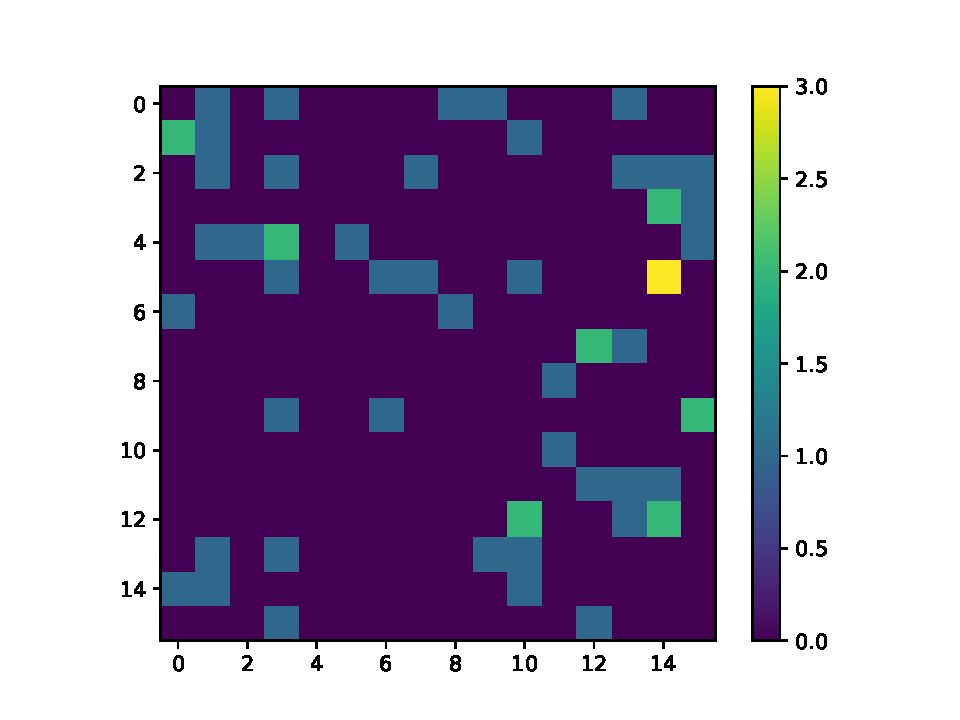
\includegraphics[width=14cm, height=9.5cm]{./Plots/5a_slice_4.pdf}
\caption{The x-y slice of the created mass grid for $z = 4$. The color indicates the assignment mass in terms of particle mass. }
\end{figure}
\newpage

\begin{figure}[!ht]
\centering
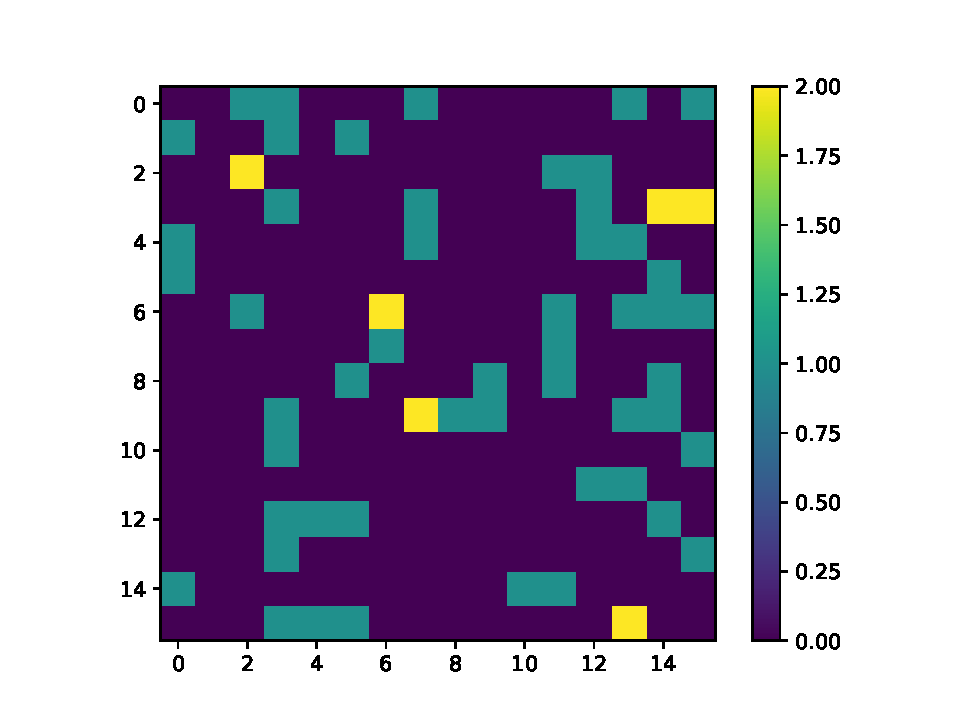
\includegraphics[width=14cm, height=9.5cm]{./Plots/5a_slice_9.pdf}
\caption{The x-y slice of the created mass grid for $z = 9$. The color indicates the assignment mass in terms of particle mass. }
\end{figure}

\begin{figure}[!ht]
\centering
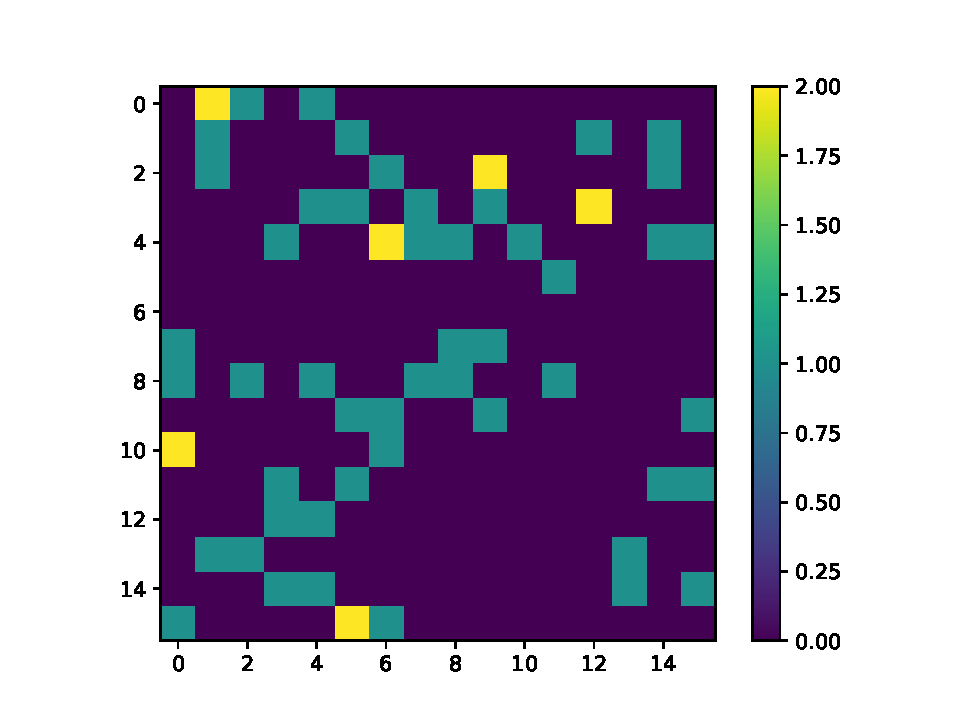
\includegraphics[width=14cm, height=9.5cm]{./Plots/5a_slice_11.pdf}
\caption{The x-y slice of the created mass grid for $z = 11$. The color indicates the assignment mass in terms of particle mass. }
\end{figure}
\newpage
\begin{figure}[!ht]
\centering
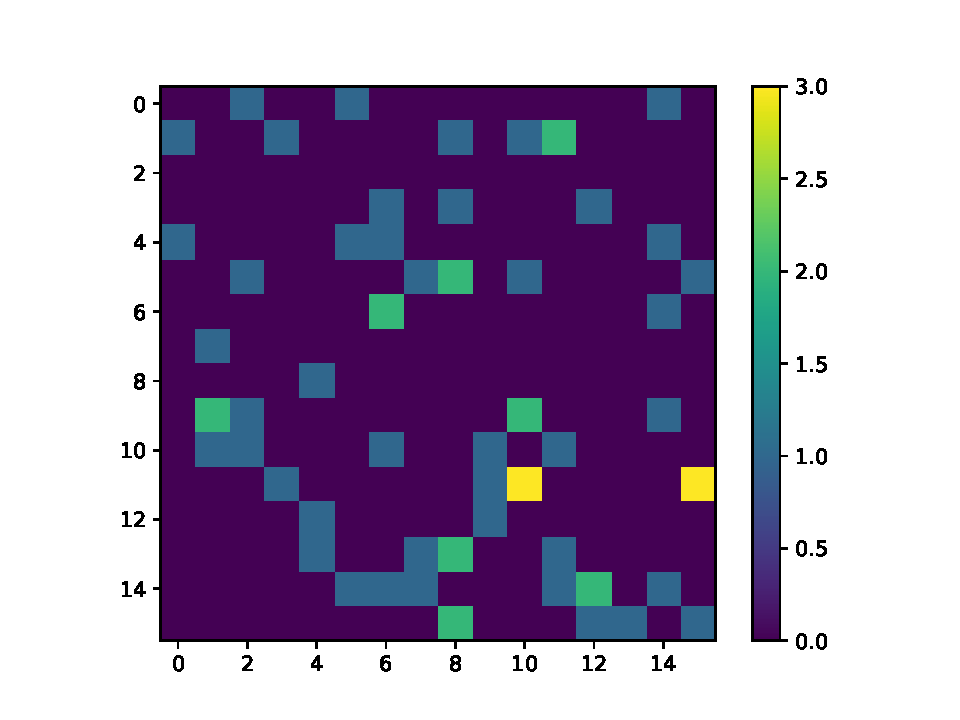
\includegraphics[width=14cm, height=9.5cm]{./Plots/5a_slice_14.pdf}
\caption{The x-y slice of the created mass grid for $z = 14$. The color indicates the assignment mass in terms of particle mass. }
\end{figure}
\end{quote}
\end{quote}











